\documentclass[14pt]{article}
\usepackage[T1,T2A]{fontenc}
\usepackage[utf8]{inputenc}
\usepackage[english,russian]{babel}
\usepackage{graphicx}
\usepackage{amsmath}
\graphicspath {{img/}}
\title{\textbf{Лабораторная работа №8\\
<<Помехоустойчивое кодирование. Декодирование методом максимального правдоподобия>>}}
\author{Перепелица А.А., ККСО-01-19}
\date{29.05.2022}
\addtolength{\topmargin}{-3cm}
\addtolength{\textheight}{3cm}
\begin{document}
\maketitle
\thispagestyle{empty}
\textbf{Цель работы:} ознакомление с принципами построения систем передачи с декодированием методом максимального правдоподобия и приобретение практических навыков постановки и проведения исследований.\\
\section{Перечень элементов на схемах}
\begin{itemize}
    \item[-] Цифровые источники питания 5В - 2 шт.; 
    \item[-] XOR2 - 18 шт.;
    \item[-] NOT - 10 шт.;
    \item[-] AND6 - 2 шт.;
    \item[-] AND2;
    \item[-] OR4 - 2 шт.;
    \item[-] OR3;
    \item[-] Ключи - 18 шт.; 
    \item[-] Дешифратор 4/16; 
    \item[-] Индикатор.
\end{itemize}
\section{Копии окон схемных файлов с позиционными обозначениями}
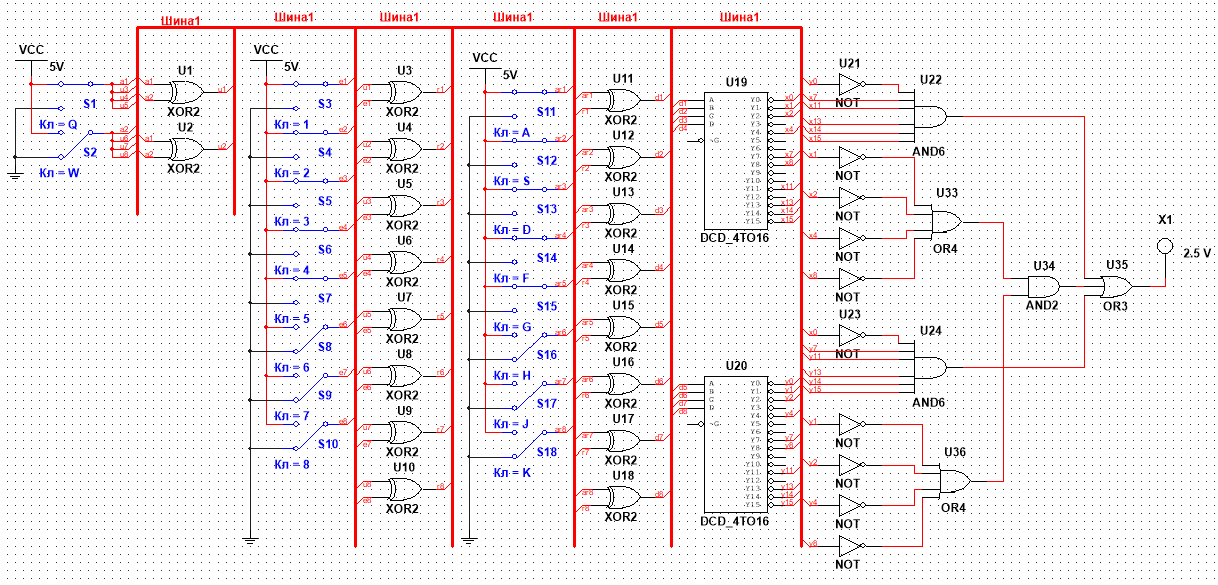
\includegraphics[width=1\linewidth]{scheme.png}
\begin{center}
    Рис. 1: Схема моделирования работы системы передачи информации с табличным декодированием группового (8,2)-кода методом максимального правдоподобия\\
\end{center}
\section{Результаты расчетов и измерения приборами}
Проведем моделирование при отсутствии и наличии помех в процессе передачи. Входная информационная последовательность $(a_{1}, a_{2}) = (1, 0)$.\\
Исходя из принципов мажоритарного кодирования имеем:\\
\begin{center}
    $U = (u_{8}, u_{7}, u_{6}, u_{5}, u_{4}, u_{3}, u_{2}, u_{1}) = (0, 0, 0, 1, 1, 1, 1, 1)$\\
\end{center}
На выходе кодера будем иметь последовательность $R = (r_{8}, r_{7}, r_{6}, r_{5}, r_{4}, r_{3}, r_{2}, r_{1})$.\\
Затем будем искать ту разрешенную последовательность, которая отстаёт от принятой комбинации R на наименьшем расстоянии.\\
\newpage
Рассмотрим на примерах:\\
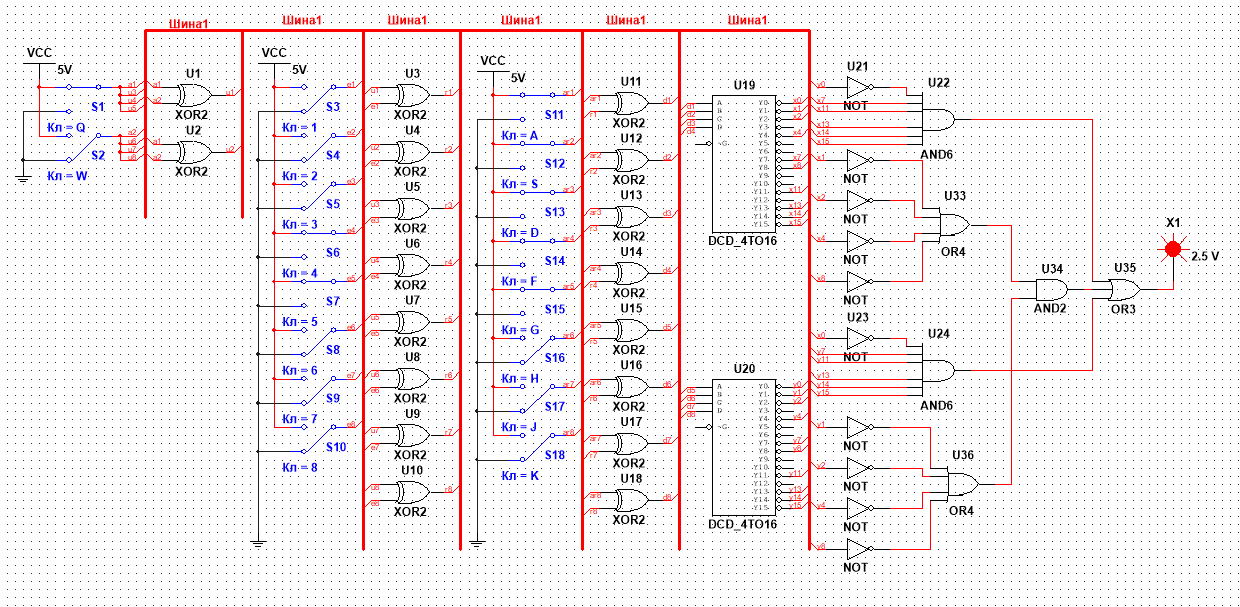
\includegraphics[width=1\linewidth]{123.png}
\begin{center}
Рис. 2: Помехи в $r_{1}, r_{2}, r_{3}$
\end{center}

Также нам понадобится таблица с разрешенными кодовыми комбинациями:\\

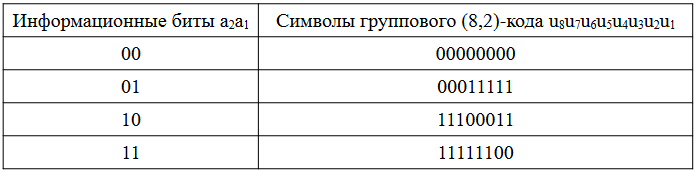
\includegraphics[width=1\linewidth]{razresh.png}

Здесь имеем:
\begin{center}
    $(a_{1}, a_{2}) = (1, 0)\\
    U = (u_{8}, u_{7}, u_{6}, u_{5}, u_{4}, u_{3}, u_{2}, u_{1}) = (0, 0, 0, 1, 1, 1, 1, 1)\\
    R = (r_{8}, r_{7}, r_{6}, r_{5}, r_{4}, r_{3}, r_{2}, r_{1}) = (0, 0, 0, 1, 1, 0, 0, 0)\\
    (a_{1}^{*}, a_{2}^{*}) = {0, 0} 
    $
\end{center}

На декодере получена последовательность $R = (00011000)$, которая ближе всего к последовательности (00000000), что соответствует информационным символам $(a_{1}, a_{2}) = (0, 0)$.\\
Рассмотрим другой пример.

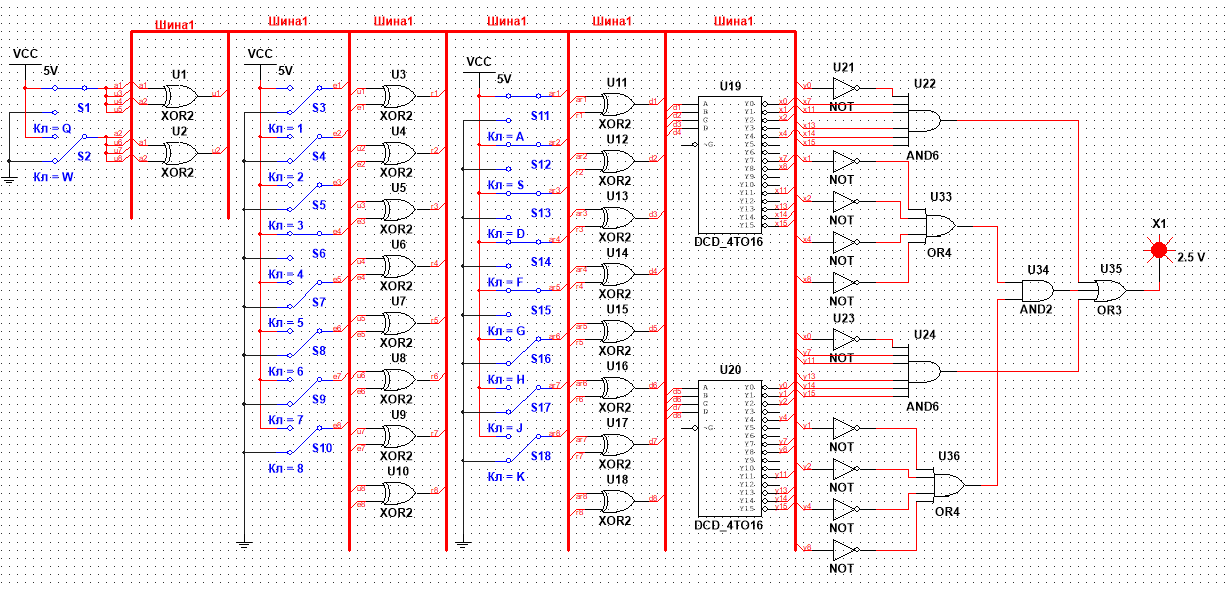
\includegraphics[width=1\linewidth]{1235.png}
\begin{center}
    Рис. 3: Помехи в $r_{1}, r_{2}, r_{3}, r_{5}$
\end{center}
Здесь имеем:
\begin{center}
    $(a_{1}, a_{2}) = (1, 0)\\
    U = (u_{8}, u_{7}, u_{6}, u_{5}, u_{4}, u_{3}, u_{2}, u_{1}) = (0, 0, 0, 1, 1, 1, 1, 1)\\
    R = (r_{8}, r_{7}, r_{6}, r_{5}, r_{4}, r_{3}, r_{2}, r_{1}) = (0, 0, 0, 1, 0, 0, 0, 0)\\
    (a_{1}^{*}, a_{2}^{*}) = {0, 0} 
    $
\end{center}

На декодере получена последовательность $R = (00010000)$, которая ближе всего к последовательности (00000000), что соответствует информационным символам $(a_{1}, a_{2}) = (0, 0)$. 

\textbf{Вывод:} в ходе работы были изучены принципы построения и работы систем передачи с использованием декодирования методом максимального правдоподобия, а также приобретены практические навыки моделирования работы при наличии помех в канале связи.
\end{document}